\section{Current-refresh surface audit}

The refreshed GLD option snapshot is separate from the Barrick equity dataset
and from the historical Team 8 parity target. At 20:15 UTC on 27 August 2026,
the provider returned 5,000 call rows; 1,912 normalized successfully, 143 met
the documented freshness, maturity, moneyness and numerical filters, and 24
structured nodes across three maturities entered the current calibration.
Eleven of the twelve requested Treasury tenors share the curve date 24 July
2026; the 10Y observation is unavailable on that date. Four isolated retries,
separated by three seconds and spanning progressively wider date windows,
returned no 24 July observation; the live provider catalogue independently
reports 1 July 2026 as the final available US10Y date. Its exclusion is
therefore a synchronous-date control rather than a throttling assumption: the
1 July point is not mixed into the 24 July cross-section. The refresh does not prove
historical market parity or predictive superiority, but it does replace the
12 August parameter objects in the unified valuation run.\cite{lse-2026}

\begin{figure}[H]
\centering
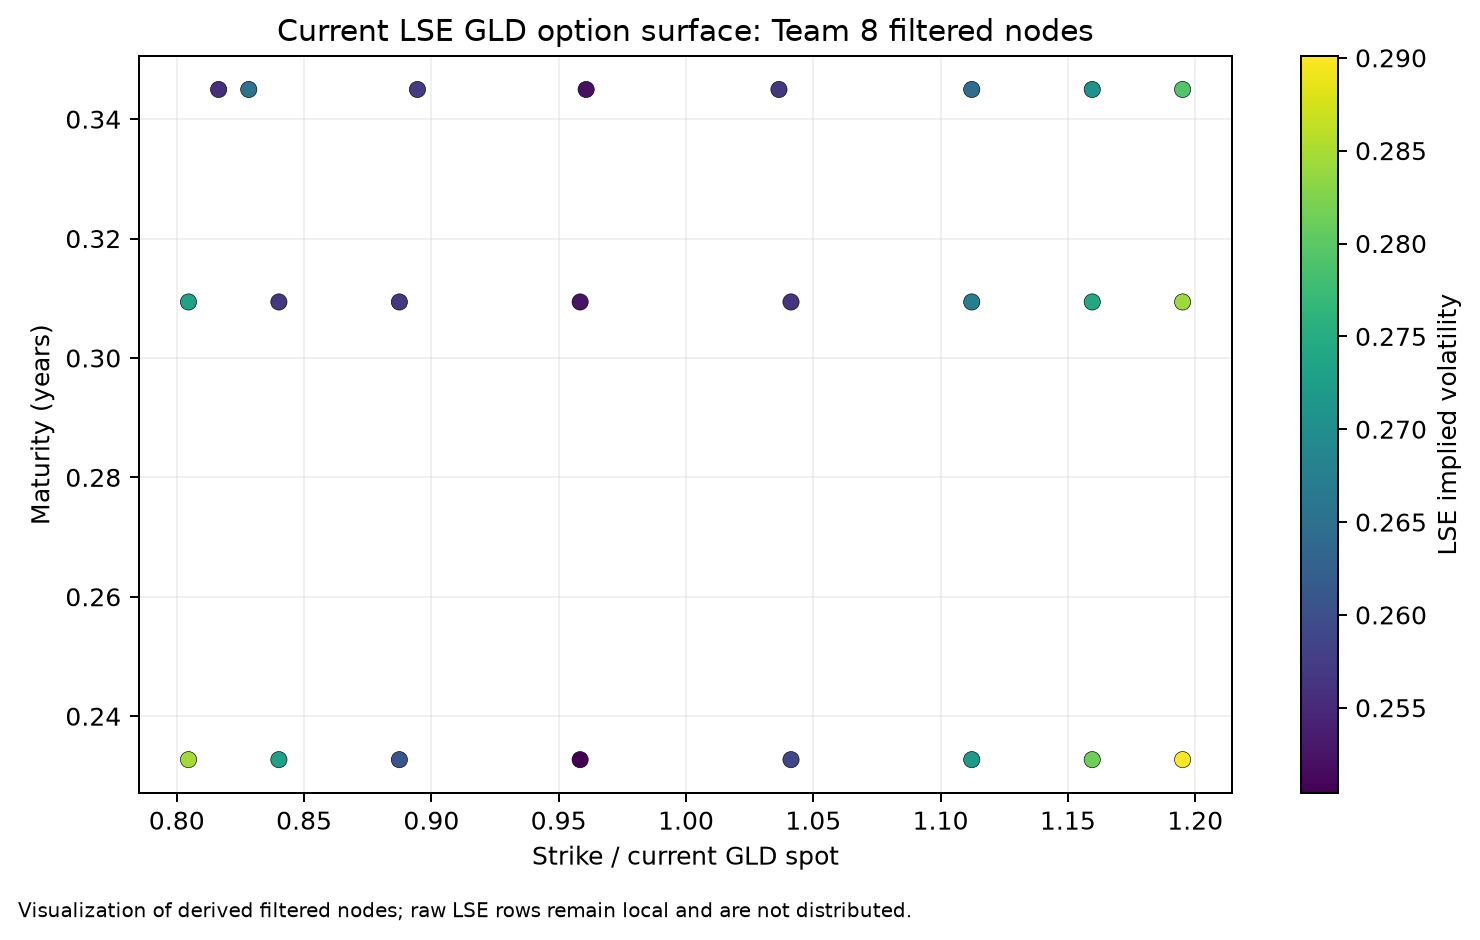
\includegraphics[width=0.88\textwidth]{img/lse/gld_option_surface_20260826.png}
\caption{Current GLD option nodes retained by the Team 8 filtering and
sampling logic. Color denotes LSE implied volatility. The surface is a
risk-neutral, IV-mapped object; it is neither a set of contemporaneous traded
prices nor a physical forecast of gold in USD/oz.}
\label{fig:gld-current-option-surface}
\end{figure}

On this 24-node sample, IV RMSE is 114.04 basis points for Black--Scholes,
86.28 for Heston, 56.55 for Bates--Poisson and 32.49 for Full
Bates--Hawkes. The richer specifications improve current in-sample fit, but
the mapped chronological source evidence still fails to establish
out-of-sample superiority over the previous-day implied-volatility surface.
Model complexity is therefore treated as a conditional representation of
option-price dynamics, not as evidence of a better physical gold forecast.
Moreover, the Full Bates--Hawkes branching ratio is 0.02, exactly the imposed
lower bound. The current cross-section therefore supports the model's combined
variance-and-jump flexibility more clearly than it identifies economically
strong self-excitation.
